\documentclass[12pt]{article}
\usepackage{fullpage,enumitem,amsmath,bbm,amssymb,amsfonts,,url,hyperref,booktabs}
\usepackage[T1]{fontenc}
\usepackage{sectsty}

\hypersetup{
    colorlinks=true,
    linkcolor=blue,
}

\sectionfont{\fontsize{15}{20}\selectfont}

\DeclareMathOperator*{\argmax}{arg\,max}
\DeclareMathOperator*{\argmin}{arg\,min}
\DeclareMathOperator{\E}{\mathbb{E}}
\usepackage{tgpagella}
\usepackage{tcolorbox}
\usepackage{forest}

\newcommand{\AK}[1]{{\bf \color{blue}AK: #1}}
\newcommand{\answer}[1]{{\bf \color{red}Answer:\\ #1}}



\begin{document}

\begin{center}
{\Large \textbf{CS224R Spring 2023 Homework 3 \\ Offline RL}}
\\ {\large Due 5/17/2023}

\begin{tabular}{rl}
SUNet ID: & $\hspace{6cm}$\\
Name: & \\
Collaborators: & 
\end{tabular}
\end{center}

\noindent By turning in this assignment, I agree by the Stanford honor code and declare
that all of this is my own work. \\
\\

\section*{Overview}

\textbf{Goals:} In this assignment you will implement two offline reinforcement learning algorithms: Implicit Q-Learning and Conservative Q-Learning. You'll be experimenting with different hyper-parameters and offline datasets that have been provided to you. Data collection is one of the most practical problems with applying Deep RL, and it's a common practice to try different exploration strategies for a given problem. In this assignment, we provide with you Random and Random Network Distillation based exploration strategies for you to compare the quality of the collected data.


You will then have the opportunity to train and tune these agents in a variety of environments in the MuJoCo physics simulator (\url{https://mujoco.org/}). 
We provide the code for generating the offline datasets as part of the assignment. Your objectives are as follows:

\begin{enumerate} 
    \item Implement and train the Conservative Q-Learning and the Implicit Q-Learning algorithms for Offline Reinforcement Learning.
    \item Experiment with the key hyperparameters for each algorithm and explore how they affect performance of your RL agents.
    \item Analyze differences between the quality of different offline data samples provided to you. 
\end{enumerate}

\vspace{0.2cm}
\noindent\textbf{Submitting the PDF}: Fill in your responses in the \texttt{answer\{\}} tags provided in the Tex template. Submit all the requested values in tables, and put in all requested plots/images as Tex figures. You should also include all your reasoning and text responses in the PDF.

\vspace{0.2cm}

\noindent\textbf{Submitting the Code and Experiment Runs}: In order to turn in your code and experiment logs, create a folder that contains the following:

\begin{itemize}
\item \texttt{data/} folder with all logged runs corresponding to both problem 1 and 2. \textbf{Note: Please remove any redundant run folders, and only keep your best run for each hyper-parameter configuration in the \texttt{data/} folder. Remove any empty/incomplete logs that correspond to interrupted/failed runs.}

\item \texttt{cs224r/} folder with all the .py files, with the same names and directory structure as the original homework repository. 
\end{itemize} 

Zip and submit the folder on Gradescope.
\vspace{0.2cm}

\noindent\textbf{Gradescope}: Submit both the PDF and the code and experiment runs in the appropriate assignment on Gradescope. An autograder will be provided to evaluate the performance of your policies from the generated tensorboard files. 

\vspace{0.2cm}

\noindent\textbf{Use of GPT/Codex/Copilot:} For the sake of deeper understanding on implementing imitation learning methods, assistance from generative models to write code for this homework is prohibited. 



\section*{Codebase}

We provide you with offline transitions dataset $\mathcal{D}$. Assuming your replay buffer has been populated with the offline dataset trajectories, your goal is to implement the corresponding reinforcement learning algorithms.

For each problem, we provide you with the files that you need to complete. Sections that need to be filled have been marked with \texttt{TODO} tags.


For this assignment, you can use the \textbf{EC c4.4xlarge} AWS instance (the instance you used for homework 2 part1). Please follow the \href{https://docs.google.com/document/d/1MpTh0BejM8Z9cQq5iCd3xUIm3mxM7viiZQIdtqkxKXw/edit?usp=sharing}{AWS Guide} for the set-up instructions. Here are the installation steps once you're on the instance. Instructions for creating the \texttt{cs224r} conda environment can be followed from homework 1.

\begin{tcolorbox}[width=\linewidth, sharp corners=all, colback=white!95!black]
\begin{verbatim}
conda activate cs224r
sudo apt-get install swig
pip install -r requirements.txt
pip install -e .
\end{verbatim}
\end{tcolorbox}



\newpage
\section*{Preliminaries}

\paragraph{Environments: } In this assignment, we'll be working with the Pointmass environment. 

The goal for the Pointmass environment is to navigate a gridworld of varying difficulties: \texttt{easy, medium} and \texttt{hard} to reach the `goal' location. Sample environments for each difficulty have been visualized in Figure~\ref{fig:pointmass_vis}

\begin{figure}[htbp]
    \centering
    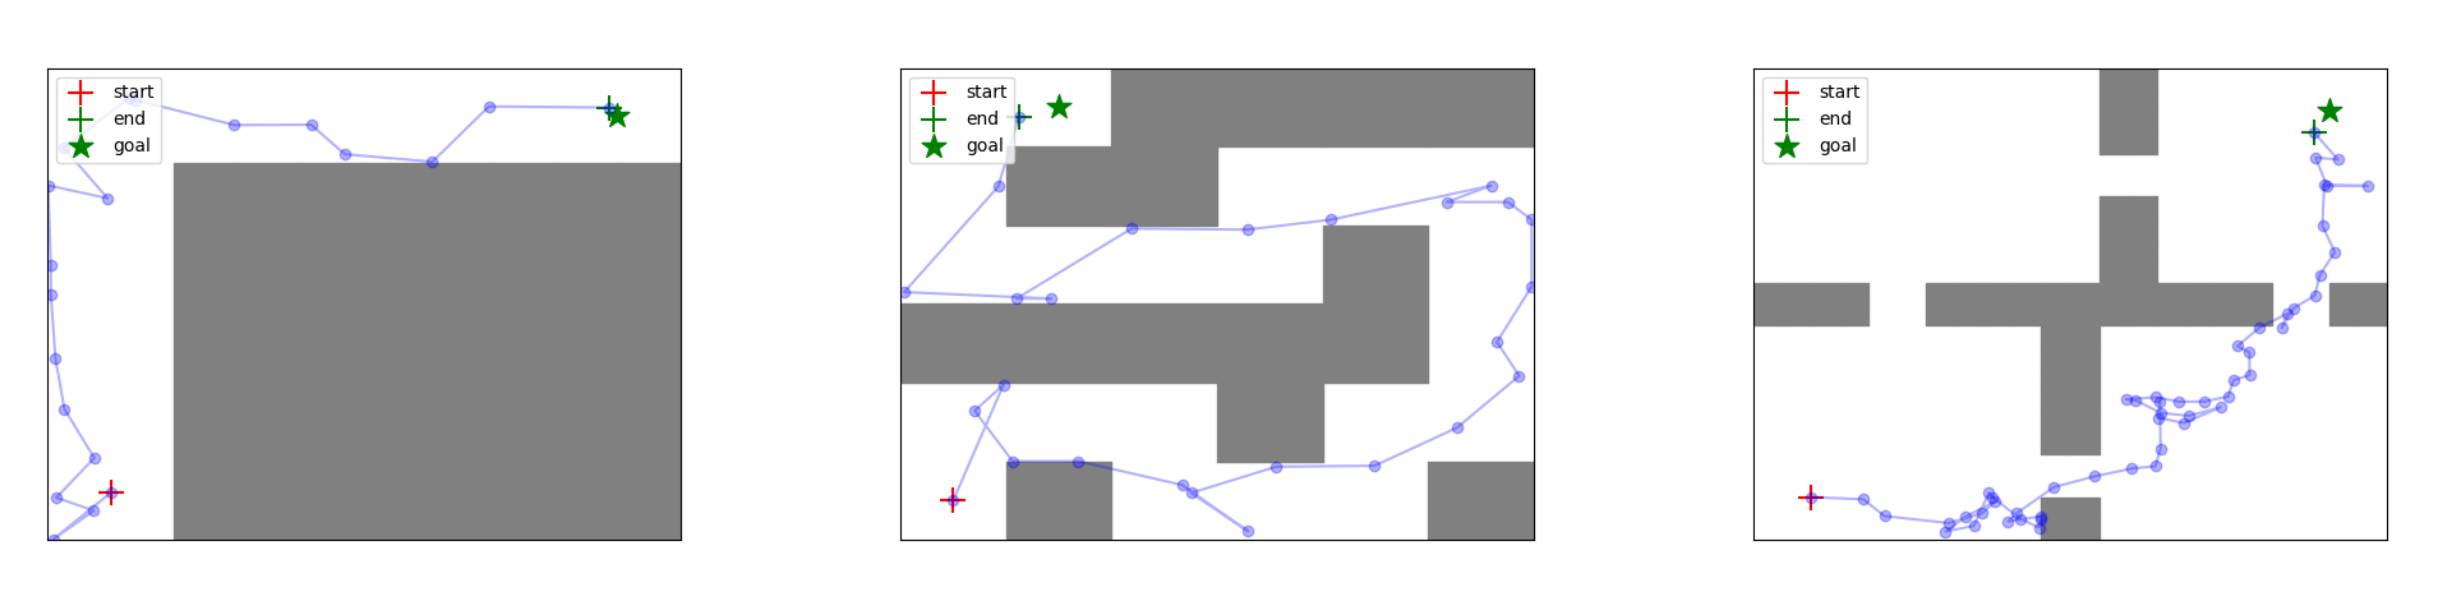
\includegraphics[scale=0.38]{figures/point_mass_envs.png}
    \caption{Visualization of the Point mass enivorment with varying difficulty levels for navigation and reaching the goal.}
    \label{fig:pointmass_vis}
\end{figure}


\paragraph{Offline datasets: } For offline RL, we have provided you with a set of exploration strategies which are used to populate the replay buffer. These trajectories then serve as the training dataset for your offline RL algorithms. In this assignment, you'll experiment with two exploration strategies (i) a Random $\mathcal{E}$-Greedy strategy and (ii) \href{https://arxiv.org/abs/2110.06169}{Random Network Distillation (RND)} algorithm. 

The RND algorithm, aims at encouraging exploration by asking the exploration policy to more frequently undertake transitions where the prediction error of a random neural network function is high. Formally, let $f_\theta^*\left(s^{\prime}\right)$ be a randomly chosen vector-valued function represented by a neural network. RND trains another neural network, $\hat{f}_\phi\left(s^{\prime}\right)$ to match the predictions of $f_\theta^*\left(s^{\prime}\right)$ under the distribution of datapoints in the buffer, as shown below:

\begin{equation}
    \phi^*=\arg \min _\phi \mathbb{E}_{s, a, s^{\prime} \sim \mathcal{D}}[\underbrace{\left\|\hat{f}_\phi\left(s^{\prime}\right)-f_\theta^*\left(s^{\prime}\right)\right\|}_{\mathcal{E}_\phi\left(s^{\prime}\right)}]
\end{equation}

If a transition $(s,a,s^\prime)$ is in the distribution of the data buffer, the prediction error $\mathcal{E}_\phi(s^\prime)$ is expected to be small. n the other hand, for all unseen state-action tuples it is expected to be large. To utilize this prediction error as a reward bonus for exploration, RND trains two critics – an exploitation critic, $Q_R(s,a)$, and an exploration critic, $Q_\mathcal{E} (s, a)$, where the exploitation critic estimates the return of the policy under the actual reward function and the exploration critic estimates the return of the policy under the reward bonus. In practice, we normalize error before passing it into the exploration critic, as this value can vary widely in magnitude across states leading to poor optimization dynamics.


\newpage
\section*{Problem 1: Implicit Q-Learning}
\begin{enumerate}
\item In this problem, you'll implement the \href{https://arxiv.org/abs/2110.06169}{Implicit Q-Learning} (IQL) method for offline RL. The actor update for IQL incorporates the advantage function similar to the actor update in the \href{https://arxiv.org/abs/2006.09359}{Advantage-Weighted Actor Critic} (AWAC) algorithm. This an advantage-weighted negative log likelihood loss function: 
\begin{equation}
    L_\pi(\psi)=-\mathbb{E}_{s, a \sim \mathcal{B}}\left[\log \pi_\psi(a \mid s) \exp \left(\frac{1}{\lambda} \mathcal{A}^{\pi_k}(s, a)\right)\right]
\end{equation}

where $\mathcal{B}$ represents samples sampled from the dataset (behavior policy that was used to collect the data). 

The actor update in AWAC corresponds to weighted maximum likelihood, where the targets are updated by reweighting the state-action pairs observed in the current dataset by the predicted advantages from the learned critic. The Q function is learnt with a Temporal Difference (TD) loss. The objective function is given below: 

\begin{equation}\label{eq:td_objective}
    \mathbb{E}_D\left[\left(Q(s, a)-r(s, a)+\gamma \mathbb{E}_{s^{\prime}, a^{\prime}}\left[Q_{\phi_{k-1}}\left(s^{\prime}, a^{\prime}\right)\right]\right)^2\right]
\end{equation}

IQL modifies the actor critic update to use expectile regression. The expectile $\tau$ of a random variable $X$ is defined as:

\begin{equation}
    \arg \min _{m_\tau} \mathbb{E}_{x \sim X}\left[L_2^\tau\left(x-m_\tau\right)\right]
\end{equation}

\begin{equation}
 L_2^\tau(\mu)= |\tau - \mathbbm{1} \{\mu \leq 0\}|    
\end{equation}
\begin{figure}[htbp]
    \centering
    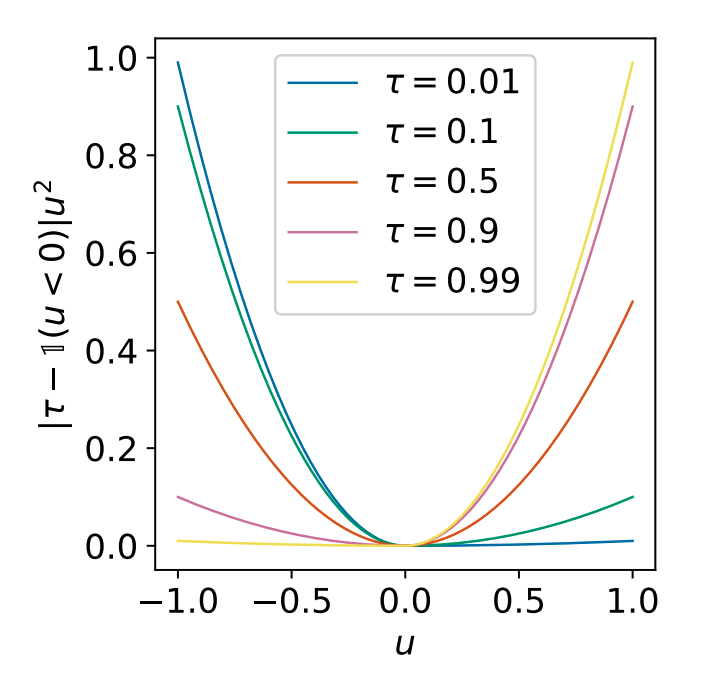
\includegraphics[scale=0.32]{figures/expectile_example.png}
    \caption{Expectile loss function visualized for different values of $\tau$.}
    \label{fig:expectile_example}
\end{figure}

That is for $\tau > 0.5$, this asymmetric loss function downweights the contributions of $x$ values smaller than $m_\tau$, while giving more weights to large values as visualized in Figure~\ref{fig:expectile_example}.



The offline dataset might contain different outcomes from similar states; in standard Q learning, we would want the critic to learn the expected value for any particular state-action pair. IQL, instead of learning the expected value, learns a given percentile. Our goal is to predict an upper expectile of the TD targets that approximate high values of $r(s, a) + \gamma * Q_\theta(s', a')$ which are present in the support of the offline dataset.

 

To perform this expectile regression, we need a separate parametric value function $V_{\phi}$. This is allows the optimization process to be differentiable, since optimizing with a single parametric q-function implies incorporating the transition dynamics as $s' ~\sim p( \cdot |s, a)$. (Note the expectation over $(s', a')$ in Equation~\ref{eq:td_objective}. Finally, the critic is \textbf{only} updated with actions that were seen in the offline dataset, and not on any out of distribution (unseen) sampled actions. This leads to the following loss functions:

\begin{equation}
    L_V(\phi)=\mathbb{E}_{(s, a) \sim D}\left[L_2^\tau\left(Q_\theta(s, a)-V_\phi(s)\right)\right]
\end{equation}

\begin{equation}
    L_Q(\theta)=\mathbb{E}_{\left(s, a, s^{\prime}\right) \sim D}\left[\left(r(s, a)+\gamma V_\phi\left(s^{\prime}\right)-Q_\theta(s, a)\right)^2\right]
\end{equation}

Fill in the TO-DOs in:
\begin{itemize}
    \item \texttt{cs224r/critics/iql\_critic.py}
    \item \texttt{cs224r/agents/iql\_agent.py}
\end{itemize}

Experiment with $\tau = 0.5, 0.9$ on the \texttt{PointmassEasy-v0} and report the eval average return and standard deviation for both cases. You can look at the final eval trajectories under the saved logs to qualitatively observe your agent's performance. The code would run for 50,000 iterations and would roughly take at most an hour to finish.  Attach the \texttt{eval\_last\_traj.png} image denoting your agent's last trajectory for each run. Which $\tau$ value performs better and why?



\begin{tcolorbox}[width=\linewidth, sharp corners=all, colback=white!95!black]
\begin{verbatim}
python cs224r/scripts/run_iql.py --env_name Pointmass{}-v0 \
--exp_name iql_tau_{}_rnd --use_rnd \
--num_exploration_steps=20000 \
--unsupervised_exploration \
--awac_lambda=1 \
--iql_expectile={}
\end{verbatim}
\end{tcolorbox}

\noindent

\answer{

}
\item Compare the learnt policies for the RND and Random exploration on the \\ \texttt{PointmassMedium-v0} environment using the best $\tau$ value from the previous runs. Report the eval average return and standard deviation. What does the performance gap between the two exploration strategies indicate about the collected data in case of offline RL?


Remove the \texttt{--use\_rnd} flag to run with random exploration:

\begin{tcolorbox}[width=\linewidth, sharp corners=all, colback=white!95!black]
\begin{verbatim}
python cs224r/scripts/run_iql.py --env_name Pointmass{}-v0 \
--exp_name iql_tau_{}_random \
--num_exploration_steps=20000 \
--unsupervised_exploration \
--awac_lambda=1 \
--iql_expectile={}
\end{verbatim}
\end{tcolorbox}

Attach the \texttt{eval\_last\_traj.png} image denoting your agent's last trajectory for each run.

\answer{
}

\end{enumerate}

\newpage

\section*{Problem 2: Conservative Q-Learning}
\begin{enumerate}
\item In this problem, you'll be implementing the \href{https://arxiv.org/abs/2006.04779}{Conservative Q-Learning} (CQL) algorithm. The goal of CQL is to prevent overestimation of the policy value. The overall CQL objective is given by the standard TD error objective augmented with the CQL regularizer weighted by $\alpha: \alpha\left[\frac{1}{N} \sum_{i=1}^N\left(\log \left(\sum_a \exp \left(Q\left(s_i, a\right)\right)\right)-Q\left(s_i, a_i\right)\right)\right]$. 

Fill in the TODOs in the following files:
\begin{itemize}
    \item \texttt{cs224r/critics/cql\_critic.py}
\end{itemize}

Once you’ve filled in all of the TODO commands, you should be able to run CQL with the following command - 
\begin{tcolorbox}[width=\linewidth, sharp corners=all, colback=white!95!black]
\begin{verbatim}
python cs224r/scripts/run_cql.py --env_name Pointmass{}-v0 \
    --exp_name cql_alpha_{}_rnd \
    --use_rnd --unsupervised_exploration \
    --offline_exploitation --cql_alpha={}
\end{verbatim}
\end{tcolorbox}

\noindent
You can look at the final eval trajectories under the saved logs to qualitatively observe your agent's performance. The code would run for 50,000 iterations and would roughly take about an hour to finish. Attach the \texttt{eval\_last\_traj.png} image denoting your agent's last trajectory for each run.  %

\noindent
Experiment with $\alpha = 0, 0.1$ on the \texttt{PointmassMedium-v0} and report the Eval average return and standard deviation for both cases on the PointmassEasy-v0 environment. What does $\alpha=0.0$ signify in terms of the algorithm? Explain the difference in obtained performance gap based on $\alpha$.

\answer{}

\item Compare the learnt policies for the RND and Random exploration on the \\ \texttt{PointmassMedium-v0} environment with $\alpha=0.1$ by reporting the eval average return and standard deviation. 
Remove the \texttt{--use\_rnd} flag to run with random exploration:

\begin{tcolorbox}[width=\linewidth, sharp corners=all, colback=white!95!black]
\begin{verbatim}
python cs224r/scripts/run_cql.py --env_name Pointmass{}-v0 \
    --exp_name cql_alpha_{}_random \
    --unsupervised_exploration \
    --offline_exploitation --cql_alpha={}
\end{verbatim}
\end{tcolorbox}


Attach the \texttt{eval\_last\_traj.png} image denoting your agent's last trajectory for each run.




\answer{}
\end{enumerate}



\end{document}
